\section{Aufbau}
\label{sec:aufbau}

Als Grundlage der hier durchgeführten Experimente dient ein virtuelles Netzwerk ausgeführt in Docker.
Dabei werden zwei Hosts (n1, n2) miteinander verknüpft.
Es ist möglich, TCP und UDP Verbindungen aufzubauen und die übertragenen Pakete in eine PCAP Datei zu speichern.
Zudem können einige Parameter für den Link zwischen den Hosts eingestellt werden.

\begin{figure}[h!]
    \centering
    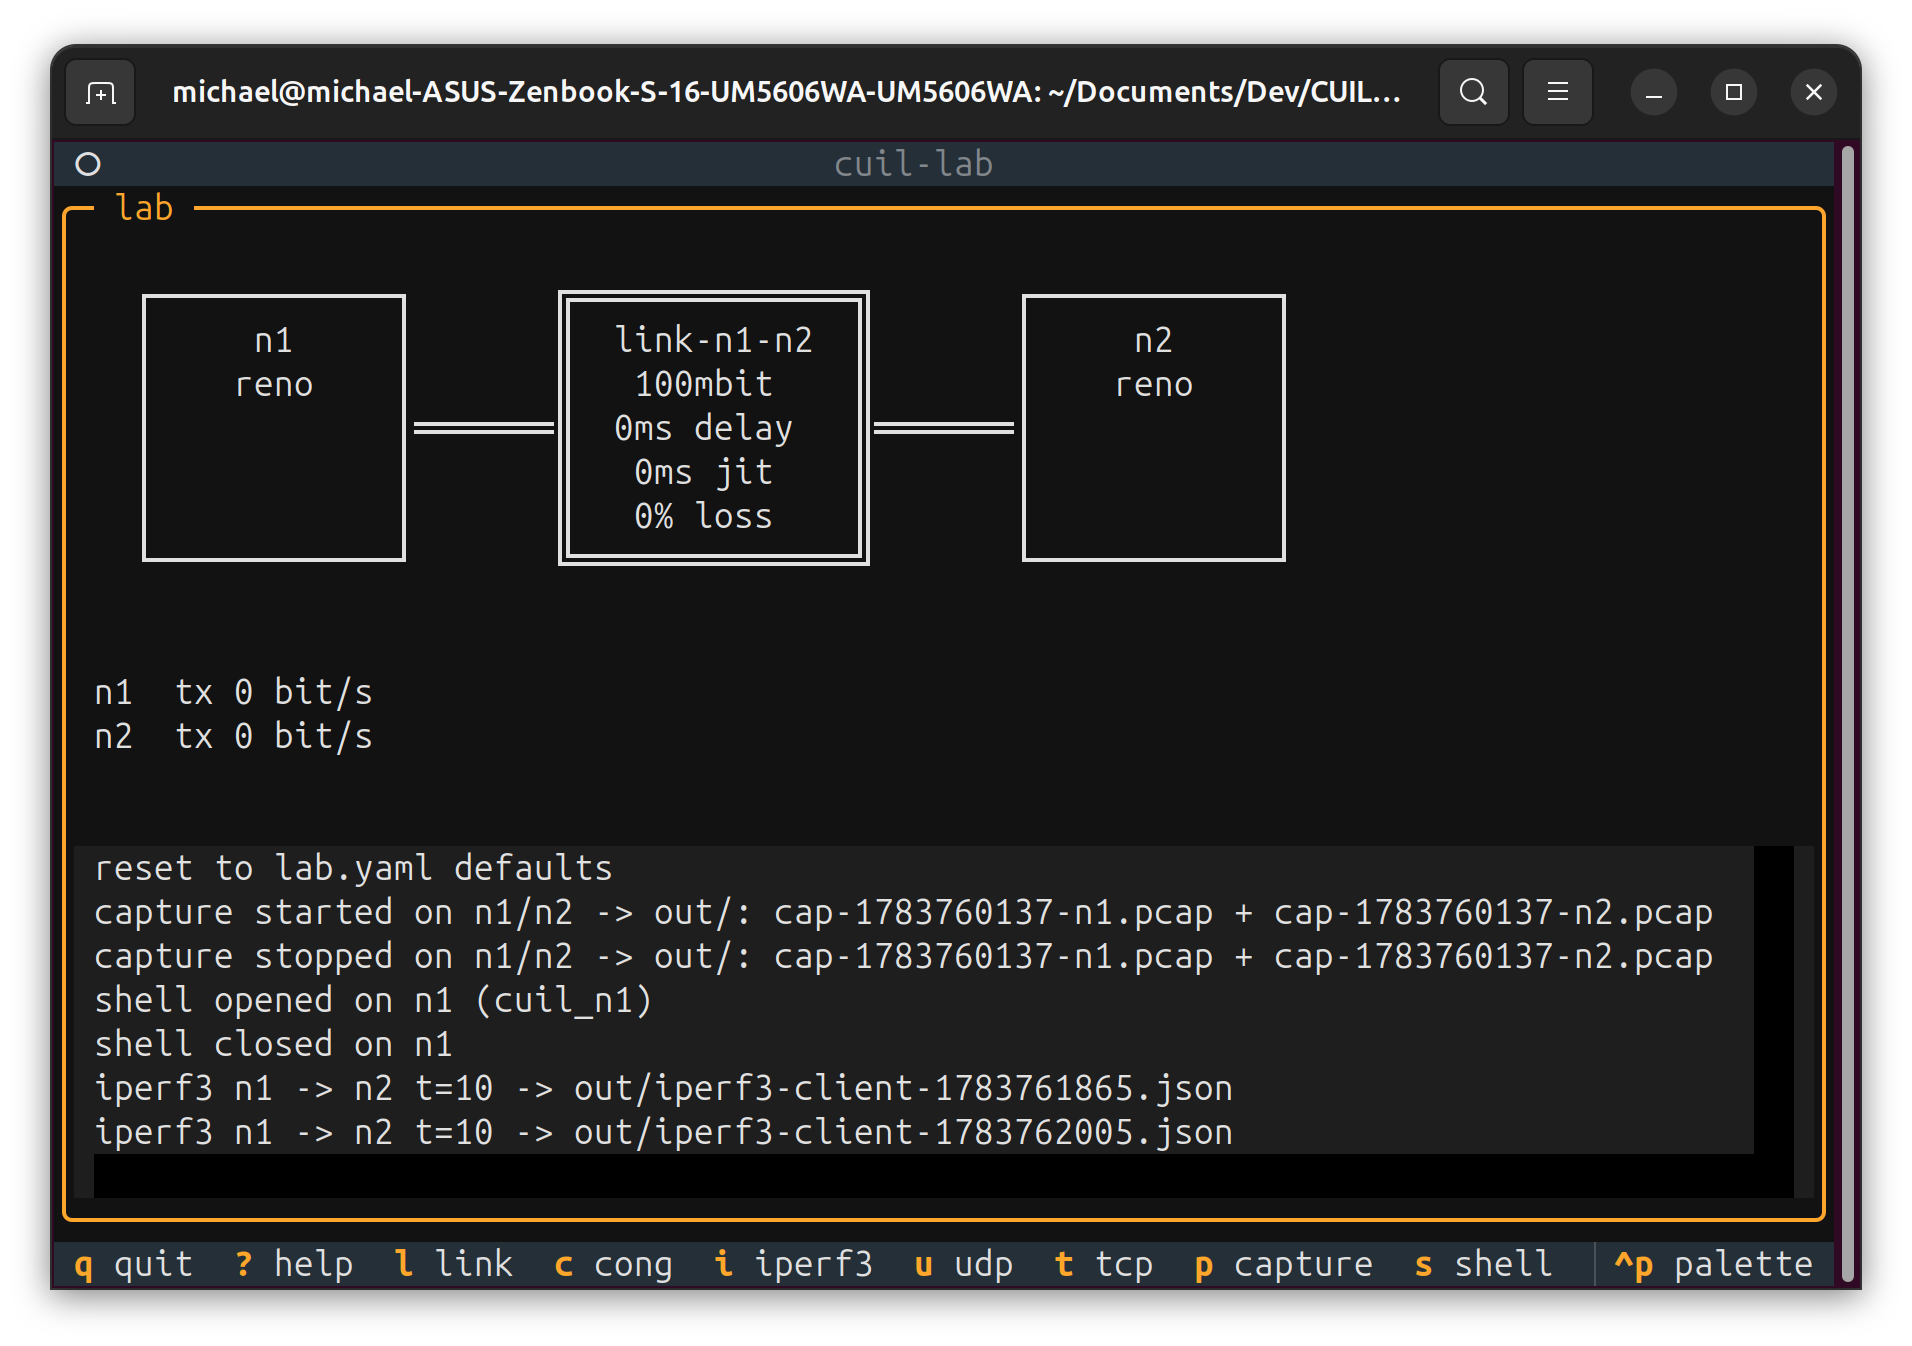
\includegraphics[width=0.9\textwidth]{figures/virtual_docker_network.png}
    \caption{Docker Netzwerk}
    \label{fig:docker_network}
\end{figure}

\subsubsection{Link Einstellungen}
\label{sec:link_einstellungen}

Der Link zwischen den Hosts kann in der Bandbreite, Latenz, Verzögerung und Paketverlust konfiguriert werden.

Standardmäßig ist der Link mit folgenden Parametern konfiguriert:
\begin{itemize}[noitemsep]
    \item Bandwidth: 100 Mbit/s
    \item Delay: 0 ms
    \item Jitter: 0 ms
    \item Paketverlust: 0 \%
    \item Burst: 32kbit
\end{itemize}

\subsubsection{TCP Staukontrolle}
\label{sec:tcp_staukontrolle_einstellungen}

Für jeden Host kann ein Standard für die Staukontrolle gewählt werden.
Zur Auswahl stehen TCP Reno und TCP CUBIC. Uns ist nicht bekannt, welcher Standard genutzt wird, da diese kontinuierlich weiterentwickelt werden.
Folgende Quellen geben einen Überblick über die beiden Staukontrollen, auch wenn sich die genaue Version des Standards unterscheiden kann.

Standardmäßig ist die Staukontrolle auf TCP Reno eingestellt.

\begin{itemize}
    \item TCP Reno: \cite{tcp_newreno}
    \item TCP CUBIC: \cite{tcp_cubic}
\end{itemize}

\subsubsection{iperf3}
\label{sec:iperf3_docker_tool}

iperf3 ist ein Tool, um Netzwerkleistung in IP Netzwerken zu messen.
Das Programm misst den Durchsatz, Paketverlust und andere Parameter \cite{iperf3}.
In der Docker Umgebung muss ein Host als Server und ein Host als Client angegeben werden anschließend noch eine Messdauer und ein Messintervall.
Eine Messung erzeugt eine JSON und eine Log-Datei, die die Ergebnisse der Messung enthalten.
In der Log-Datei ist zu sehen, dass für jedes Intervall gemessen wird wie viele Daten übertragen wurden, daraus ergibt sich der gemessene Durchsatz und die Übertragungsrate für den Link.

\subsubsection{udp}
\label{sec:udp_docker_tool}

Das UDP Tool in der Docker Umgebung kann genutzt werden, um UDP Verbindungen zwischen den Hosts aufzubauen.
Dabei müssen Server und Client angegeben werden, sowie die Anzahl der Pakete, das Intervall und die Paketgröße.
Beim Ausführen sendet der Client UDP Pakete an den Server. Für den ganzen Vorgang wird eine Log-Datei pro Endpunkt erstellt, die die Anzahl der gesendeten und empfangenen Pakete enthält.

Die Standardeinstellungen für das UDP Tool sind:
\begin{itemize}[noitemsep]
    \item Server: n2
    \item Client: n1
    \item Count: 10
    \item Interval: 0.1 s
    \item size: 64 B
\end{itemize}

\subsubsection{tcp}
\label{sec:tcp_docker_tool}

Das TCP Tool in der Docker Umgebung kann genutzt werden, um TCP Verbindungen zwischen den Hosts aufzubauen.
Dabei müssen Server und Client angegeben werden, sowie die Anzahl der Pakete, das Intervall und die Paketgröße.
Zusätzlich zu diesen Einstellungen, die wir auch für UDP nutzen, kann eingestellt werden, ob eine persistente Verbindung genutzt werden soll, oder ob für jedes Paket eine neue Verbindung aufgebaut werden soll.

Die Standardeinstellungen für das TCP Tool sind:
\begin{itemize}[noitemsep]
    \item Server: n2
    \item Client: n1
    \item Count: 10
    \item Interval: 0.1 s
    \item size: 64 B
    \item Mode: persistent
\end{itemize}

\subsubsection{PCAP Capture}
\label{sec:pcap_docker_capture}

In der Docker Umgebung ist es möglich, die übertragenen Pakete in eine PCAP Datei zu speichern.
Dazu kann ein Capture mit p gestartet werden.
Anschließend wird pro Host eine PCAP Datei erstellt, die alle Pakete enthält, die über den Link übertragen wurden bis das Capture wieder gestoppt wird.

\subsubsection{Shell} \label{sec:shell_docker_tool}

In der Docker Umgebung ist es möglich, eine Shell auf den Hosts zu öffnen.
Mit der Shell können Hosts konfiguriert und Befehle ausgeführt werden, die nicht über die Docker Umgebung möglich sind.
